% !TeX spellcheck = pl_PL

\newpage
\part{Zadania}

% ==================================================
% --- ETHERNET
% ==================================================
\section{Ethernet}
	% ================= ZADANIE 1 ==================
	\subsection{Zadanie}
		\subsubsection{Treść}
			Kontroler karty sterownika sieci Ethernet odebrał następujące ramki:
			\begin{enumerate}
				\item Długość 51 bajtów, poprawne CRC
				\item Długość 39 bajtów, błędne CRC
				\item Długość 66 bajtów, poprawne CRC
				\item Długość 1510 bajtów, poprawne CRC
				\item Długość 1525 bajtów, poprawne CRC
				\item Długość 1540 bajtów, błędne CRC
			\end{enumerate}
			Jak zaklasyfikować powyższe ramki? (błąd protokołu, błąd transmisji, kolizja, poprawna ramka)
		\subsubsection{Odpowiedź}
			\begin{itemize}
				\item Jeśli ramka ma mniej niż 64 bajty i błędne CRC to jest to kolizja
				\item Jeśli ramka ma mniej niż 64 bajty i poprawne CRC to jest to błąd protokołu
				\item Jeśli ramka ma więcej niż 1518 bajtów, to zawsze jest to błąd protokołu, niezależnie od poprawności CRC
				\item Jeśli ramka ma niemniej 64 bajty i nie więcej niż 1518 bajtów oraz niepoprawne CRC to jest to błąd transmisji
				\item Poprawna ramka powinien mieć 64 - 1518 bajtów i poprawne CRC
			\end{itemize}
			\begin{enumerate}
				\item Błąd protokołu
				\item Kolizja
				\item Poprawna
				\item Poprawna
				\item Błąd protokołu
				\item Błąd protokołu
			\end{enumerate}
	% ================= ZADANIE 2 ==================
	\subsection{Zadanie}
		\subsubsection{Treść}
			W przypadku wystąpienia kolizji w segmencie sieci Ethernet czas oczekiwania na retransmisję $ T_R $ generowany jest jako liczba losowa z przedziału:
			\begin{enumerate}
				\item O stałej wielkości ustalanej przy konfiguracji sieci (jakiej?)
				\item O wielkości rosnącej liniowo z numerem kolizji
				\item O wielkości rosnącej z kwadratem numeru kolizji
				\item O wielkości rosnącej z kwadratem do pewnego numeru kolizji
			\end{enumerate}
			Jak obliczany jest czas $ T_R $?
		\subsubsection{Odpowiedź}
			Chodzi tutaj o algorytm CSMA, wykorzystywany do rozwiązywania kolizji na łączu kablowym. Wzór, o który prosi pytanie, zawarty jest w algorytmie dostępu w transmisji częściowo kontrolowanej. W pełni kontrolowanym dostępie występuje Token oraz rywalizacja stacji o dostęp (chyba o to chodzi).
			$$ T_{R} = r(x)\times (2^{k}-1)\times T_{ob}$$Gdzie:
			\begin{itemize}
				\item $ r(x) $ - liczba losowa z zakresu 0...1
				\item $ T_{ob} $ - czas obiegu łącza, w najgorszym wypadku podwojony czas propagacji
				\item $ k $ - liczba kolizji, czyli który raz się te ramki już zderzyły.
				\item Wraz ze zwiększaniem się liczby kolizji, możliwy zakres rośnie ekspotencjalnie. Jednak maksymalna wielkość $ k $ jest równa \textbf{10}. Dla $ k > 10 $ przyjmuje się $ k=10 $.
				\item Próbujemy szczęścia aż $ k < 15 $, potem próby są przerywane.
			\end{itemize}
			Dlatego poprawna odpowiedź to: \textit{Czas oczekiwania na retransmisję $ T_R $ generowany jest jako liczba losowa z przedziału \textbf{o wielkości rosnącej z kwadratem do pewnego numeru kolizji, \underline{a tym numerem jest 10}}}\\
			{\small \emph{Forczu: jeszcze to sprawdzę}}.
			
% ==================================================
% --- ROUTING
% ==================================================
\section{Routing}
	% ================= ZADANIE 1 ==================
	\subsection{Zadanie}
		\subsubsection{Treść}
			\begin{wraptable}{r}{5.5cm}
				\begin{tabular}{|c|c|}
					\hline \multicolumn{2}{|c|}{Q}  \\ 
					\hline \multicolumn{2}{|c|}{1}  \\ 
					\hline \multicolumn{2}{|c|}{300}  \\ 
					\hline T & 2 \\ 
					\hline U & 1 \\ 
					\hline Z & 3 \\ 
					\hline 
				\end{tabular}
			\end{wraptable}
			Węzeł Q generuje co 60 sekund pakiety Link State, w chwili $ t_0 $ rozesłał pakiet
			$$ (Q\;|\;seq=23321\;|\;age=300\;|\;(U|3)\;|\;(V|2)\;|\;(Z|5)\;) $$
			Po restarcie w chwili $ t_0+25\;s $ wysłał pakiet
			$$ (Q\;|\;seq=1\;|\;age=300\;|\;(T|2)\;|\;(U|1)\;|\;(Z|3)\;) $$
			a potem kolejne. Przedstaw przebieg dystrybucji tej informacji w sieci. Kiedy te zmiany w topologii zostaną uwzględnione w wyznaczaniu tablicy routingu?
		\subsubsection{Odpowiedź}
			Działanie Link State:
			\begin{itemize}
				\item Nr sekwencyjny - jeśli ktoś dostanie pakiet o większym numerze, to go przetwarza, a jeśli nie jest większy, to nie.
				\item Wiek - czas życia pakietu (w cyklu). Jeśli czas życia upływa to jest usuwany z tablicy routingu. Liczony w sekundach.
			\end{itemize}
			\textbf{Odpowiedzi}:
			\begin{enumerate}
				\item Węzły odrzucają pakiet z niższym numerem sekwencyjnym, więc nowy pakiet będzie uwzględniony po wygaśnięciu wa(żności?) pierwszego, czyli za $ 275\;s $.\\
				\small{ \emph{Ocenione na 0.9 / 1.0}}
				\item W momencie restartu, po 25 sekundach, oba pakiety żyją i ważniejszy jest Pierwszy z nich, o numerze sekwencyjnym $ seq=23321 $. Dlatego pakiet o $ seq=1 $ zostanie uwzględniony po przedawnieniu $ seq=23321 $, czyli po:
				$$ 300 - 25 - t_0\;[s]= 275\;[s] $$
				a najpierw zostanie wykorzystany pakiet o $ seq=23321 $.
				\item \emph{by Forczu}: tablica po uwzględnieniu pakiet o $ seq=23321 $ \\
					\begin{tabular}{|c|c|}
						\hline \multicolumn{2}{|c|}{Q}  \\ 
						\hline \multicolumn{2}{|c|}{1}  \\ 
						\hline \multicolumn{2}{|c|}{300}  \\ 
						\hline T & 2 \\ 
						\hline U & 1 \\
						\hline V & 2 \\
						\hline Z & 3 \\ 
						\hline 
					\end{tabular}\\\\
				Nowe $ U=3 $, czyli koszt jest wyższy od obecnego, więc nie jest uwzględnione.\\
				Nowe $ Z=5 $, czyli to samo co wyżej.\\
				Nowe $ V=5 $, tego nie ma w obecnej tablicy, więc po prostu jest dodane.
		\end{enumerate}
			
\section{Transmisja danych}
	% ================= ZADANIE 1 ==================
	\subsection{Zadanie}
		\subsubsection{Treść}
			Stacja robocza podłączona jest z serwerem łączem o przepustowości $ 55\;Mbit/s $, z bitową stopą błędów $ BER=4.9\cdot 10^{-6} $. określ, ile czasu zajmie przesłanie tym łączem pliku 100 kB danych, od nawiązania do zakończenia połączenia protokołem TCP w wersji standardowej, jeśli uzgodniona maksymalna wielkość segmentu wynosi 1024 B (ramki o łączu 1082 B), wielkość okna odbiorcy wynosi 17 kB, a czas RTT wynosi 25 ms.
		\subsubsection{Odpowiedź}
			$ BER=4.9\cdot 10^{-6} $
			\begin{itemize}
				\item Oznacza to, że 4.9 bitu zostaje przekłamanych na 1 milion bitów.
				\item Czyli 4.9 bajtów zostaje przekłamanych na 12500 bajtów.
			\end{itemize}
			Wielkość okna odbiorcy: 17 kB = 17000 B\\
			Wielkość segmentu: 1024 B\\
			Ramka w łączu: 1082 B\\
			Maksymalna liczba ramek w jednym przesyle:
			$$ \lfloor\frac{17000\;[B]}{1082\;[B]}\rfloor = 15$$
			Przepustowość = $ 55\;Mbit/s $
			$$ SRET=\frac{23\cdot 1024\;[B]}{5\cdot 25\;ms}=18841600\;[\cfrac{B}{S}] $$
			Do przesłania: 100 kB danych = 102400 B\\
			Czas wysłania 100 kB danych:
			$$ \frac{102400\;[B]}{18841600\;[\frac{B}{S}]}\approx0.00054\;s$$
			\small{ \emph{Forczu: jakoś tak, nie widać wszystkiego, jeszcze się poprawi.}}

\section{Adresacja}
	% ================= ZADANIE 1 ==================
	\subsection{Zadanie}
		\subsubsection{Treść}
			Jak przebiega (po raz pierwszy w danych środowisku) proces tłumaczenia nazwy na adres IP dla nazwy daisy.sales.euro.hp.com? Czy zwracany wynik i proces tłumaczenia różni się czymś przy drugiej próbie w stosunku do pierwszej (odstęp między żądaniami kilka minut, pierwsza zakończona pomyślnie)? Jak będzie przebiegał późniejszy o kilka minut proces tłumaczenia nazwy dino.support.americas.hp.com?
		\subsubsection{Odpowiedź}
			\begin{enumerate}[A]
				\item 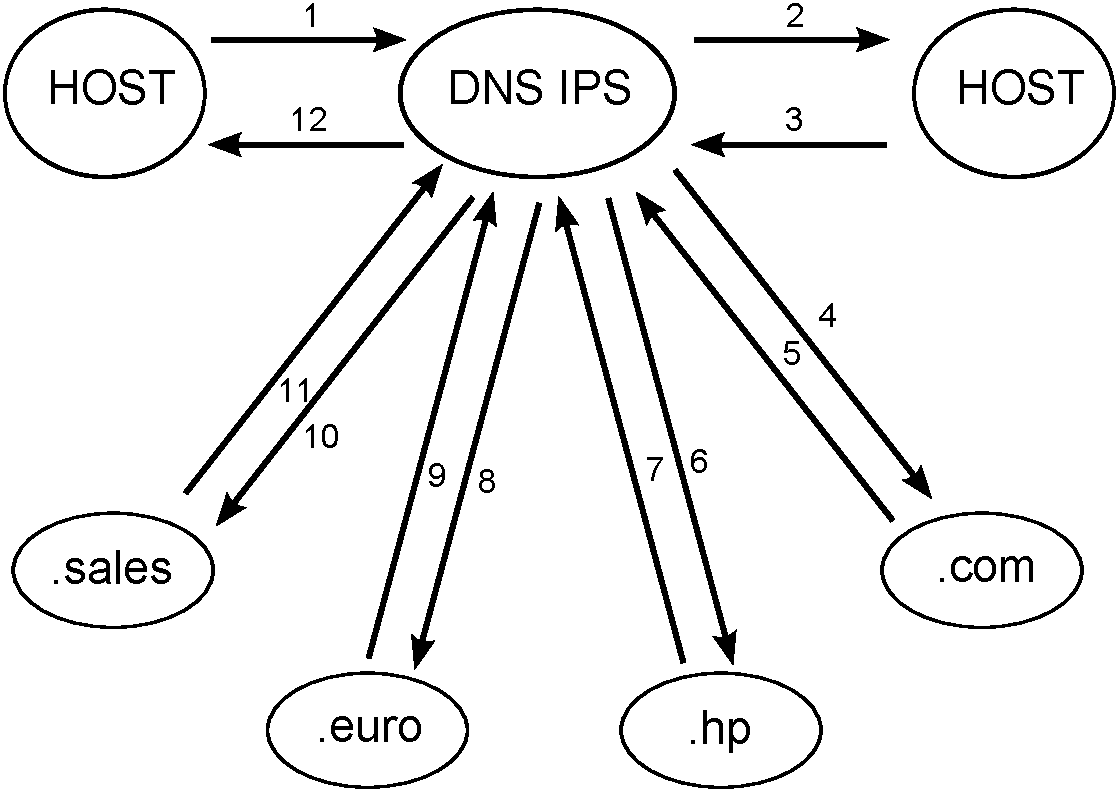
\includegraphics[width=6cm]{./images/zadanie01.pdf}\\
				\begin{enumerate}[1]
					\item Zapytanie DNS o adres IP dla daisy.sales...
					\item Jeśli DNS nie posiada tego adresu to pyta root server
					\item Ten odpowiada, że nie zna adresu IP dla daisy.sales.euro.hp.com , ale zna adres dla com i ... (przekierowuje)
					\item DNS ISP pyta dns com o daisy.sales.euro.hp.com
					\item Ten odpowiada, że go nie zna, ale zna adres dla hp
					\item DNS ISP pyta dns hp o daisy.sales.euro.hp.com
					\item Ten odpowiada, że go nie zna, ale zna adres dla euro
					\item DNS ISP pyta dns euro o daisy.sales.euro.hp.com
					\item Ten odpowiada, że go nie zna, ale zna adres dla sales
					\item DNS ISP pyta dns sales o daisy.sales.euro.hp.com
					\item Serwer sales zwraca adres IP domeny daisy.sales.euro.hp.com. Następnie DNS ISP p(...) go do hosta.
					\item ...
				\end{enumerate}
				\small{ \emph{Brak pełnej treści, ale ocenione na 1.0 / 1.0}}
				\item
					\begin{enumerate}
						\item daisy.sales.euro.hp.com.root
						\begin{enumerate}[1]
							\item Zapytanie do NS .com czy "zna" .hp
							\item Zapytanie do NS .hp czy zna .euro
							\item Zapytanie do NS .euro czy zna .sales
							\item Zapytanie do NS .sales czy zna .daisy
							\item Otrzymanie adresu IP
						\end{enumerate}
						W drugim przypadku adres hp.com może nie być tłumaczony.
						\item dino.support.americas.hp.com
						\begin{enumerate}[1]
							\item Znamy IP (hp.com), pytamy czy zna .americas
							\item Zapytanie do NS czy zna .support
							\item Zapytanie do NS czy zna .dino
							\item Otrzymanie adresu IP
						\end{enumerate}
					\end{enumerate}
					\small{ \emph{Ocenione na 1.0 / 1.0}}
			\end{enumerate}
			

\section{Poczta e-mail}
	% ================= ZADANIE 1 ==================
	\subsection{Zadanie}
		\subsubsection{Treść}
			Przedstawić z jakich elementów składa się koperta przesyłki poczty elektronicznej.
			\begin{enumerate}[a)]
				\item Jak przebiega i który z protokołów poczty elektronicznej odpowiada za jej przekazanie?
				\item Jak przebiega odbiór przesyłki przez adresata, który z protokołów obsługuje tę operację?
			\end{enumerate}
		\subsubsection{Odpowiedź}
			\begin{enumerate}[a)]
				\item List elektroniczny wysyłany jest za pomocą protokołu SMTP. Klient inicjuje połączenie poleceniem "helo". Następnie podaje adres nadawcy "mail from", adres odbiorcy "rcpt to", treść listu "data". Kończy poleceniem "quit".
				\item Listy odbierane są za pomocą protokołów POP3. Klient żąda listy wiadomości poleceniem "list". Następnie pobiera cały żądany list i usuwa go z serwera : "Retr" i "Dele". Sesja kończy się poleceniem "quit". Oczywiście zanim to wszystko nastąpi musi zostać przeprowadzona autentyfikacja. Klient POP3 zaczyna sesję od podania nazwy użytkownika "user" i hasła "pass".
			\end{enumerate}
			\small{ \emph{Ocenione na 1.0 / 1.0}}
